\documentclass[11pt]{article}

% --- Packages ---
\usepackage{amsmath, amssymb}
\usepackage{graphicx}
\usepackage{float}
\usepackage{natbib}
\usepackage{lineno}
\usepackage{hyperref}
\usepackage{xcolor}
\usepackage{fullpage}
\usepackage{titlesec}

\linespread{1.7}

% --- Section formatting (optional, keep if you want consistency) ---
\titleformat{\section}[block]{\Large\bfseries}{\thesection}{1em}{}
\titleformat{\subsection}[block]{\large\bfseries}{\thesubsection}{1em}{}

% --- Line numbering ---
\linenumbers
\modulolinenumbers[3]

% --- Title ---
\title{Supplementary Materials: Additional Methods, Analyses, and Simulations}

\author{
	Alexandra Campbell$^{1,\dagger}$ (ORCID: 0009-0008-4893-8029) \and
	Tom E.X. Miller$^{1,\ast}$ (ORCID: 0000-0003-3208-6067)
}

\date{}

\begin{document}
	
	\maketitle
	
	
	
	
	\appendix
	\label{appendix}
	\section{Additional Methods and Parameters} \label{appendix:A}
	\renewcommand{\thefigure}{A\arabic{figure}}
	
	In addition to the models described in the body of the paper, we fit several other models using data from previous studies.
	These models are described below.
	
	\paragraph{Seeds Per Fruit}
	With data from \cite{Miller2007}, we fit a model for the number of seeds produced by every fruit on a cholla ($\kappa(a')$) in year $t+1$ based on the ant partner $a'$ in year $t+1$.
	We fit this model to seed data $y^{\kappa}$ using a Negative Binomial distribution and the log link function: 
	$$y^{\kappa} \sim  Negative Binomial(\hat{\kappa},\hat{\phi})$$
	$$\hat{\phi} = \beta_{0}^{\phi}$$
	The data used for this model did not include data on ants in the ``other" category, so we used the data from vacant plants to parameterize seeds per flower for plants with ``other" ants in the IPM.
	
	\begin{figure}
		%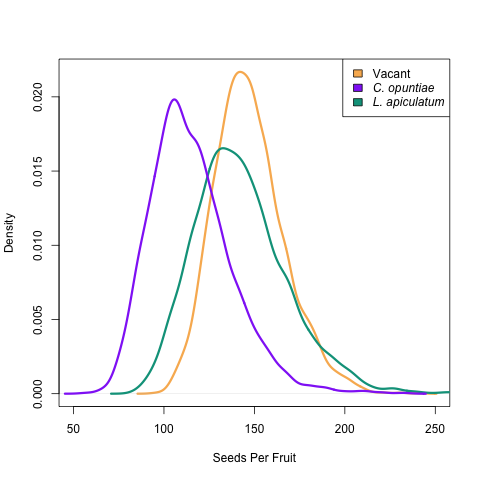
\includegraphics[width=0.91\linewidth]{Figures/Seeds_Per_Fruit.png}
		\caption{
		}
		\label{app:seeds}
	\end{figure}
	
	
	We found that vacant plants produced the most mean seeds (147.2 per fruit), followed by \textit{L. apiculatum} tended plants (142.4 per fruit), and finally, \textit{C. opuntiae} tended plants (115.0 per fruit).
	
	
	\paragraph{Recruit Size Distribution}
	We fit this model to recruit size data $y^{\eta}$ using a Normal distribution with the identity link function: 
	$$y^{\eta} ~\sim N(\hat{\eta},\hat{\sigma})$$
	where $\hat{\sigma}$ is estimated with a non-informative prior. 
	
	We found that the mean size of recruits is $log(-2.097) m^3$ with an interquartile range from $log(-2.173) m^3$ to $log(-1.712) m^3$.
	
	
	
	\paragraph{Germination}
	With germination data \cite{Miller2009}, we fit two models for the probability of germinating from the first year seedbank ($\gamma_1$) or the second year seedbank ($\gamma_2$) in year $t+1$, with no fixed or random effects.
	These models were fit to germination data $y^{\gamma_1}, y^{\gamma_2}$  using the binomial distribution with logit link functions:
	$$y^{\gamma_1} \sim Binomial(\hat{\gamma_1})$$
	$$y^{\gamma_2} \sim Binomial(\hat{\gamma_2})$$
	
	We found that the mean germination rates for seeds in the seedbank for one year  is 0\%, with an interquartile range of 0\% and 1\%.
	We found that the mean germination rates for seeds in the seedbank for a second year is 0\%, with an interquartile range of 0\% to 0.4\%.
	Seeds are more likely to germinate in their first year in the seedbank, but most seeds will never germinate. 
	
	\paragraph{Pre-Census Survival}
	With recruit census data \cite{Miller2006}, we fit a model for the probability of a seedling (which germinates in early Fall) surviving to when we census in May ($\delta$) of year $t+1$ (accounting for missed mortality events), with fixed effects of the previous size $x$ and random effects of the transect $m$.
	We fit this model to pre-census survival data $y^{\delta}$ using a Bernoulli distribution with a logit link function: 
	$$y^{\delta} ~ Bern(\hat{\delta})$$
	where $m \sim N(0, \sigma_{transect}^2)$ is the random effect of transect where the recruited individual was analyzed for survival.
	
	We found that plants have a 16.2\% probability of surviving from germination to the next census.
	Our model estimated this very well, expecting a 16.3\% probability.
	
	%% Reproduction Model
	\paragraph{Probability of Flowering}
	We fit a model for the probability of flowering ($P$) in year $t+1$ based on the size ($x$) in year $t+1$ with random effects of year $\tau_a$ using a Bernoulli distribution with a logit link function: 
	$$y^{P}~ Bern(\hat{P})$$
	$$\hat{P_i} = \beta^0 x_i + \tau_{a[i]}$$
	
	\begin{figure}
		%	
\includegraphics[width=0.91\linewidth]{Figures/repro_panel.png}
		\caption{}
		\label{app:repro}
	\end{figure}
	
	
	\begin{figure}
		%
\includegraphics[width=0.91\linewidth]{Figures/flow.png}
		\caption{ }
		\label{app:flow}
	\end{figure}
	
	The probability of a plant reproducing in a given year is highly size dependent. 
	The mean probability of reproducing remains at about 0\% until the plant reaches a medium size, after which the mean probability of reproducing increases steadily before reaching about 100\% at large sizes (Figure \ref{app:repro}). 
	
	\paragraph{Number of Flowers Produced}
	We fit a model for the flowers produced ($F$) in year $t+1$ based on the size ($x$) in year $t+1$ with random effects of year $\tau_a$ using a zero truncated negative binomial distribution: 
	$$y^{F}~ Bern(\hat{F})$$
	$$\hat{F_i} = \beta^0  x_i + \tau_{a[i]}$$
	
	The number of flowers produced by a reproducing plant is also highly size dependent. 
	The mean number of flowers produced are 0 until the plant reaches a medium size, after which the mean number of flowers produced increases to about 45 at the largest sizes (Figure \ref{app:flow}).
	
	
	
	
	
	
	
	\section{Observed Herbivory Data} \label{appendix:B}
	\renewcommand{\thefigure}{B\arabic{figure}}
	
	Herbivory is an important driver in this population and shapes the range and demography of cholla.
	Herbivore presence has been shown to negatively impact growth and fecundity of cholla populations \citep{Miller2009}.
	Ant visitors are believed to offer defensive benefits to the plants they tend in this system, leading to the hypothesis that ant presence would be correlated with reduced herbivory.
	Therefore, herbivore protection is the likely driver behind the increased survival, growth, and reproductive rates of tended plants. 
	Fluctuations in herbivore communities across time would also lead to potentially important fluctuations in ant visitor responses and therefore cholla demographic responses.
	
	Here we conduct  an analyses of herbivory levels on plants with different ant visitors and contrast them to herbivory levels on plants with no visitors.
	Evidence that herbivory is decreased for tended plants further strengthens the results presented in the main text that ant presence is beneficial.
	
	Herbivory data was collected during annual demographic censuses. 
	This involved noting the type and quantity of herbivores observed. 
	Presence of herbivores is considered to be herbivore pressure as it is assumed they will damage the plant if they are present.
	This data has been taken consistently since 2014, so the analysis below considers 9 years of data.
	We considered only plants which were reproducing, since prior work shows that flowering significantly elevates herbivore pressure \citep{Miller2006}.
	The proportion of reproducing plants that experienced herbivory was calculated for each ant state separately.
	Analysis showed that ant presence is correlated with lower herbivore visitation.
	We observed herbivores on 40\% of vacant cacti.
	Plants tended by Other ants experienced similar, though lower, frequency of observed herbivores on reproducing plants (herbivores detected on 37.5\% of plants).
	Herbivores were detected on 25\% of plants tended by \textit{C. opuntiae} ants and on 11\% of plants tended by \textit{L. apiculatum} ants.
	These results indicate that ant presence is correlated with lower levels of herbivory and that partner identity has an impact on the level of herbivory.
	They also indicate that the partner correlated with the lowest levels of herbivory is \textit{L. apiculatum} ants.
	These findings are consistent with literature findings which show that \textit{L. apiculatum} ants are the most aggressive (therefore the most effective against herbivores) \citep{Miller2007}.
	
	
	\begin{figure}[H]
		%
\includegraphics[width=0.7\linewidth]{Figures/herb_all.png}
		\caption{}
		\label{app:herb}
	\end{figure}
	
	
	
	\section{Alternative Ant Transition Simulations}\label{appendix:C}
	\renewcommand{\thefigure}{C\arabic{figure}}
	
	In addition to the competitive exclusion model defined and analyzed in the body of the paper, we simulated results from several other potential models. 
	We chose to include competitive exclusion as our primary results in the paper because we believe it to be the most biologically realistic.
	However, in building and testing of alternative models we found that the method of ants occupying plants significantly impacts the fitness of the population. 
	We tested two alternative transition models, one called the frequency based model and one called the equal likelihood model. 
	
	\paragraph{Frequency Based Model}
	The first alternative hypothesis we tested was what we called the frequncy based model.
	In this model rather than the proportion of vacant cacti being maintained, the proportion of cacti occupied by each species is maintained and when one is removed it is replaced with vacancy.
	This version of the model assumes that the frequency of each ant we see is reflective of the real frequency of populations rather than some other mechanism.
	With this model we found very clear evidence of Sampling Effect in the system. 
	When only  \textit{C. opuntiae}, Other ants, or both ants are present, there is very little difference in the fitness of the cacti from when no partners are present. 
	Only when \textit{L. apiculatum} ants are present do we see an increase in the fitness of the focal mutualist (Figure \ref{app:FreqLambdaMeans}a).
	In this simulation, the more partners that are present the higher the fitness of the focal mutualist is, confirming that partner diversity would be beneficial through sampling effect if this transition model were correct.  (Figure \ref{app:FreqLambdaMeans}b).
	
	
	\begin{figure}
		%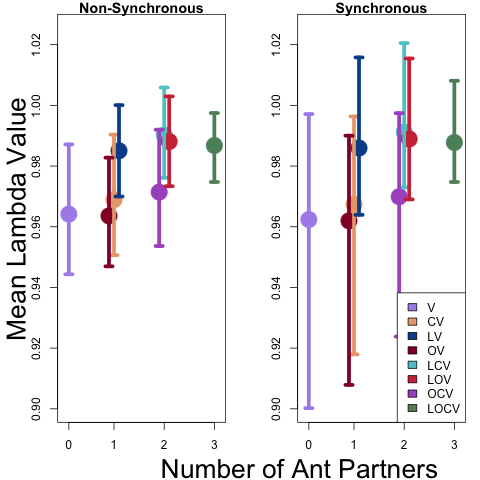
\includegraphics[width=0.91\linewidth]{Figures/Lambdas_Freq_lines.png}
		\caption{}
		\label{app:FreqLambdaMeans}
	\end{figure}
	
	\paragraph{Equal Likelihood Model}
	The second alternative hypothesis we tested was what we called the equal likelihood model.
	In this model we preserved the observed pattern of size-dependent vacancy/occupancy, but occupancy was manipulated to be equally likely for all partner identities. 
	This was designed to remove the effect overwhelming numbers of \textit{L. apiculatum} ants may have. 
	Despite very different proportions, we found very similar outcomes to the competitive exclusion model analyzed in the paper. 
	All ants are beneficial, but having more than one is not necessarily any better than having an individual species as a partner (Figure \ref{app:EqualLambdaMeans}b).
	Partner presence is beneficial, but neither identity nor number of partners appears to be important (Figure \ref{app:EqualLambdaMeans}a).
	
	\begin{figure}
		%\includegraphics[width=0.91\linewidth]{Figures/Lambdas_equal_lines.png}
		\caption{}
		\label{app:EqualLambdaMeans}
	\end{figure}
	
	
	\section{The Portfolio Effect} 
	\label{appendix:D}
	\renewcommand{\thefigure}{D\arabic{figure}}
	
	This appendix includes our evaluation of evidence for the portfolio effect under realistic conditions (those observed in the field) as well as simulated conditions.
	
	\paragraph{Portfolio Effect Evidence}
	We compared the effects of partner diversity (estimated as $\lambda_S^4 - \lambda_S^0$) for the synchronized and non-synchronized models.
	We determined that non-synchronous effects of ant partners are greater than synchronous effects of ant partners only 50\% of the time.
	This means there is no evidence of portfolio effect in this system.
	
	
	\begin{figure}[H]
		%	
\includegraphics[width=\linewidth]{Figures/portfolio_effect.png}
		\caption{}
		\label{fig:Portfolio}
	\end{figure}
	
	
	To further evaluate the potential for a portfolio effect, we conducted an additional analysis in which we increased the degree of difference among ant partners. 
	Specifically, we manipulated the correlation structure of ant-specific year random effects in the stochastic IPM. 
	In the first scenario, we forced the correlation among ant species to be zero, representing complete independence of partner responses across years. 
	In the second scenario, we forced the correlation as close to -1 as possible, representing maximally anti-correlated partner responses.
	To reach a zero correlation and a maximally negative one, we reordered the vector of mean ant-specific year random effects in each year so that high values for one ant corresponded to low values for another, and vice versa, while preserving the original distribution of effects. 
	We continued reordering each vector until the correlations reached the desired values. 
	The resulting manipulated vectors allowed us to evaluate the fitness of the cacti under different partner diversity scenarios when the ants experienced different asynchronous responses to inter-annual fluctuations, allowing us to determine if portfolio effect was possible under different ant conditions.
	
	
	For each of these scenarios, we quantified the effect of partner diversity as the difference between projected population growth with no partners and with the full suite of partner diversity ($\lambda_S^4 - \lambda_S^0$), and compared results under synchronous versus non-synchronous environmental variation. 
	Both scenarios resulted in greater benefits of partner diversity under non-synchronous conditions, though the evidence was much stronger when the ants were anti-correlated, as expected under the portfolio effect hypothesis. 
	This shows that portfolio effect is possible in this system if the ant partners diverged more greatly in their responses to annual variation.
	
	
	\begin{figure}
		%	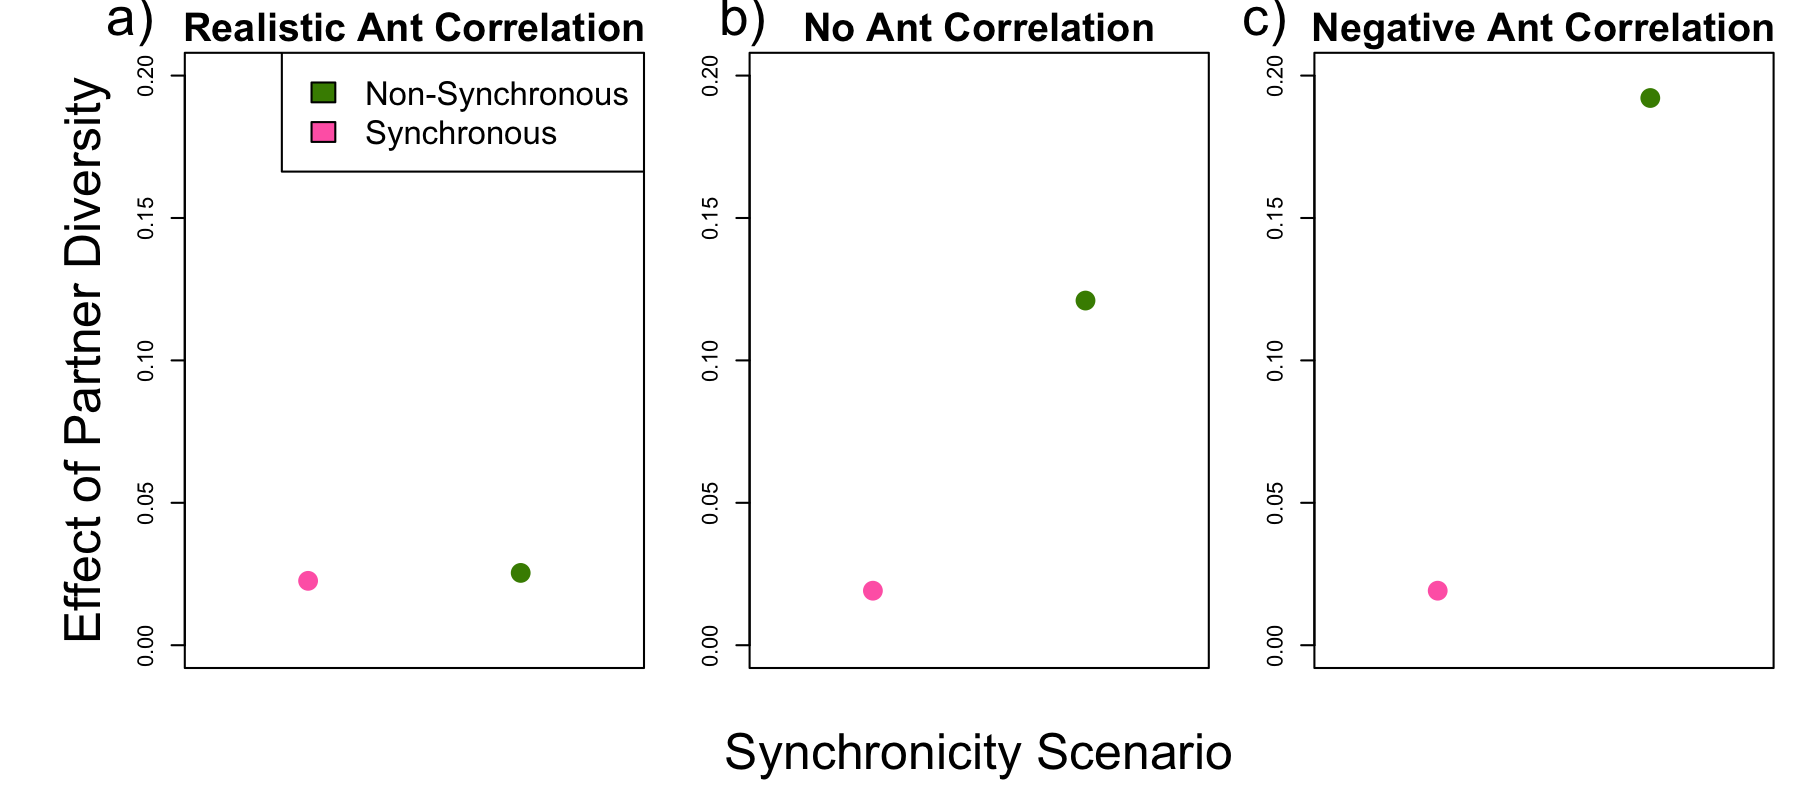
\includegraphics[width=0.91\linewidth]{Figures/cor0_Portfolio_Effect.png}
		\caption{
		}
		\label{app:portfolio}
	\end{figure} Help me make this a separate PDF in latex (a new document)
	
\end{document}